\documentclass[a4paper, 11pt]{article}
%\usepackage[utf8]{inputenc}
\usepackage{appendix}
\usepackage{listings}
\usepackage{color}
\usepackage{xcolor}
\usepackage{float}
\usepackage[british]{babel}
\usepackage{amsmath}
\usepackage{amsfonts}
\usepackage{amssymb}
\usepackage{amsthm}
%\usepackage{amsrefs}
\usepackage{enumerate}
\usepackage{graphicx}
\usepackage{caption}
\usepackage{subcaption}
\usepackage{url}
\usepackage[round]{natbib}
\usepackage[all]{xy}
\usepackage{tikz}
\usepackage{hyperref}
\usepackage[percent]{overpic}
\usepackage[printwatermark]{xwatermark}
\usepackage{epstopdf}
\usepackage{fancyvrb}
\usepackage{longtable}
\usepackage{wasysym}
%\usepackage{multicol}
\usepackage{pgfplots}
%\usepackage{newtxtext,newtxmath}
%\newwatermark[allpages,color=red!20,angle=45,scale=4,xpos=0,ypos=0]{DRAFT}

%\usepackage{antpolt}
%\usepackage[T1]{fontenc}
%\usepackage{tocloft}
\usepackage{selinput}
\SelectInputMappings{
  adieresis={ä},
  edieresis={ë},
  idieresis={ï},
  udieresis={ü},
  eacute={é},
}

\newcommand{\widefigwidth}{\textwidth}
\newcommand{\mgraphheight}{.21\textheight}

\usetikzlibrary{positioning}

\definecolor{MidnightBlue}{RGB}{11,28,121}
\definecolor{dkgreen}{rgb}{0,0.6,0}
\definecolor{mauve}{rgb}{0.58,0,0.82}

\newcommand{\citeneed}{{\color{red} [citation needed] }}
\newcommand{\citepos}{{\color{orange} [citation needed?] }}
\newcommand{\todo}[1]{{\color{red} TODO:} {\color{dkgreen} #1}}
\newcommand{\ennl}[1]{{\color{red} \it [TL: #1]}}

\newcommand{\Python}{\texttt{Python}}

\renewcommand{\thefigure}{\arabic{section}.\arabic{figure}}

\newcommand{\mat}[1]{\left(\begin{matrix} #1 \end{matrix} \right)}
\newcommand{\HRule}{\rule{\linewidth}{0.5mm}}
%\renewcommand{\cftdot}{}
%\renewcommand{\cftsecleader}{\cftdotfill{\cftdotsep}}
\setcounter{tocdepth}{3}

\usepackage{tikz}
\usetikzlibrary{shapes,arrows}

\floatstyle{ruled}
\newfloat{example}{htb}{lop}
\floatname{example}{Example}
\newfloat{codeblok}{htb}{lop}
\floatname{codeblok}{Codeblok}

%\newcommand{\citep}[1]{\cite{#1}}\newcommand{\citet}[1]{\cite{#1}}
\renewcommand{\cite}[1]{\citep{#1}}

\renewcommand{\lstlistingname}{Codeblok}
\lstdefinestyle{lstjava}{
language=Java,
numbers=left,
numberstyle=\tiny\color{red},
stepnumber=5,
numbersep=5pt,
tabsize=2,
breaklines=true,
keywordstyle=\color{MidnightBlue},
commentstyle=\color{dkgreen},
stringstyle=\color{mauve},
morekeywords={}
}
\lstdefinestyle{lstmatlab}{
language=Matlab,
numbers=left,
numberstyle=\tiny\color{red},
stepnumber=5,
numbersep=5pt,
tabsize=2,
breaklines=true,
keywordstyle=\color{MidnightBlue},
commentstyle=\color{dkgreen},
stringstyle=\color{mauve},
morekeywords={linreg,linregquad,logreg,ones,repmat}
}
\lstnewenvironment{lstmat}{
\lstset{style=lstmatlab}}{}

\lstnewenvironment{lstsource}{
\lstset{
language=C,
breaklines=true,
showspaces=false,
showstringspaces=false,
showtabs=false,
morekeywords={}
}}{}

\lstdefinestyle{lstcpp}{
language=C++,
numbers=left,
numberstyle=\tiny\color{red},
stepnumber=5,
numbersep=5pt,
tabsize=2,
breaklines=true,
keywordstyle=\color{MidnightBlue},
commentstyle=\color{dkgreen},
stringstyle=\color{mauve},
morekeywords={}
}


\title{Automatic Plastic Soup Solver\\ {\Large Project plan}}
\author{student: \\Ysbrand Galama \\ 10262067 \and supervisor: \\ Thomas Mensink}
\date{\today}

\begin{document}
\maketitle

\section{Problem definition} 
Large amounts of plastic waste end up in the world's oceans and have a big impact on the marine life \citep{barnes2005drifting}.
A collective noun for this environmental problem is Plastic Soup or Plastic Ocean.
Because the plastic does not decay in nature, a lot of marine life gets the plastic in their digestive system. Figure \ref{fig:plastic-bird} shows how much plastic can end up in a bird.

\begin{figure}[h!bt]
\centering
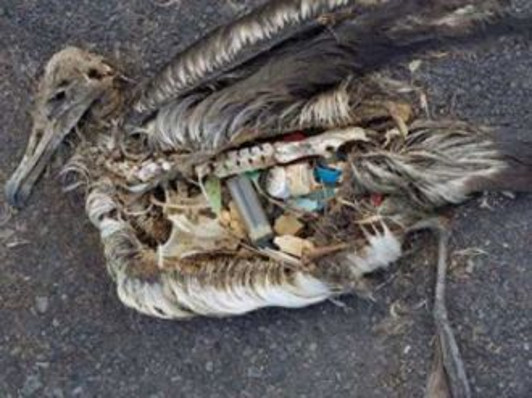
\includegraphics[keepaspectratio=true,width=.5\textwidth]{images/Bird_with_plastic_stomach.jpg}
\caption{The stomach contents of a bird that ate plastic}
\label{fig:plastic-bird}
\end{figure}

Several organisations are working on solving this environmental hazard.
One of them is Saraswater.
They are developing ships that shovel the plastic from the water.
This project could help to make a system that can automate that process.
If an autonomous agent could detect from cameras where the plastic is, the ships could be controlled by this agent to clean it up.

This project would start the development of this autonomous agent by giving it ``eyes''. The main question is how the current state-of-the-art techniques in image recognition could be used to detect floating plastic in the ocean.
Because of the current accuracy of Convolutional Neural Networks (CNN) \citep{razavian2014cnn}, this project will start with them as a baseline.
This project does not have the amount of data or resources to train a deep learning CNN. Therefore a pre-trained network will be used, which brings the question:
{\it
How does a pre-trained CNN perform when used for other classifications without being trained on a large amount of domain-specific data?
}


\section{Literature Review}
%\subsection{Convolutional Neural Networks}
In the Machine Learning the Convolutional Neural Network (CNN) has existed for quite some time \citep{fukushima1980neocognitron}. However, due to computational complexity is was only recently that \citet{krizhevsky2012imagenet} showed an implementation to compute large CNNs.
\citeauthor{krizhevsky2012imagenet} implement a CNN on a computers GPU that can work with the massive parallelism necessary to compute many layers of nodes.

This technique is currently popular with image recognition tasks. From large amounts of data, an accurate recognition system can be trained \citep{girshick2014rich}, \citep{razavian2014cnn}.
The dataset in this project is small with only 40k images. Therefore training a CNN will not be possible. However, because of the manner a CNN is build, it will not be necessary to fully train the network. The bottom layers of a CNN trained on large image datasets detect basic visual concepts, for instance lines and simple shapes. Only higher in the network the concepts become more abstract and less local \citep{zeiler2014visualizing}.
Therefore it should be possible to replace the last layer of a pre-trained CNN with a layer trained on this dataset, which is what this project will research.

%The state-of-the-art technique that will be used in this project comes from \citet{krizhevsky2012imagenet}. To understand the CNN better, \citet{zeiler2014visualizing} will help. Moreover, \citet{girshick2014rich} and \citet{razavian2014cnn} show that applying a CNN is a promising baseline to start.

%\paragraph{Textures} Besides the CNN, this project will also research the diferent texture recognition techniques and their application on the Plastic Soup image data. Local binary patterns \citep{guo2010completed} and local derivative patterns \citep{zhang2010local} will be used in this case. Probably a combination of a CNN with these techniques will be used.

%\paragraph{Other imagery techniques} On the usage of fisher vectors, \citet{sanchez2013image} is a place to start. The colour model of \citet{van2010evaluating} will be used, as will the possibilities of Colour SIFT \citep{ai2010color}


\section{Method and Approach}
A dataset has been collected by separating the frames of short clips filmed by Bill MacDonnald on the plastic soup problem. This data has been cleaned and annotated by hand which gave a total set of 37165 images. The data has been split in 16553 images above and 20612 images below water, from which 20635 images show plastic only, 6972 images show animals only and 8502 images show both. In figure \ref{fig:plastic-data} example images are shown.

\begin{figure}[h!bt]
\centering
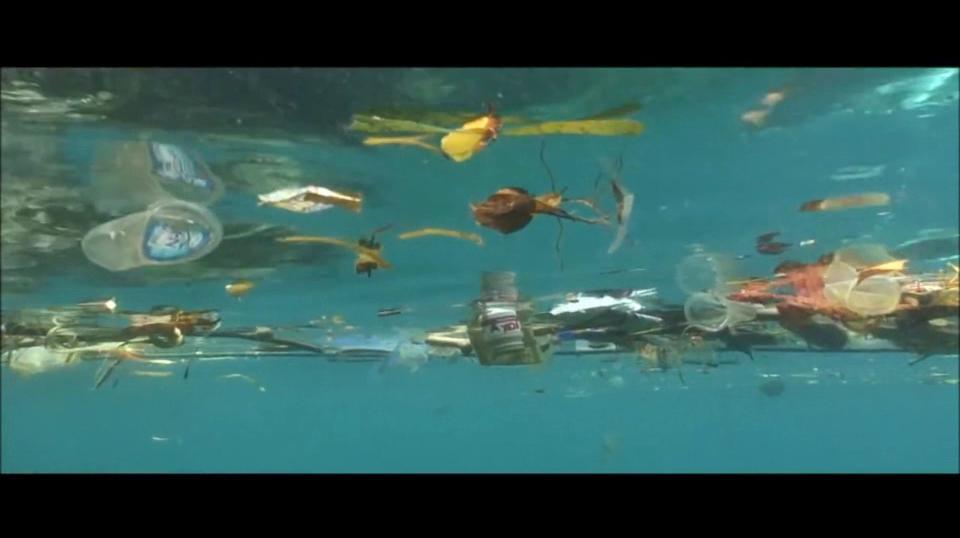
\includegraphics[keepaspectratio=true,width=.5\textwidth]{images/10947_01.jpg}\\
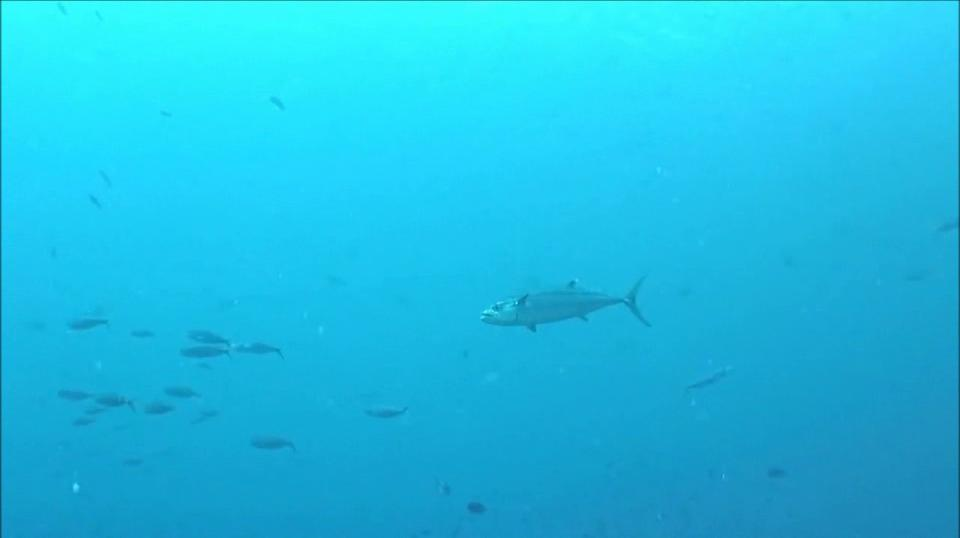
\includegraphics[keepaspectratio=true,width=.5\textwidth]{images/19358_10.jpg}\\
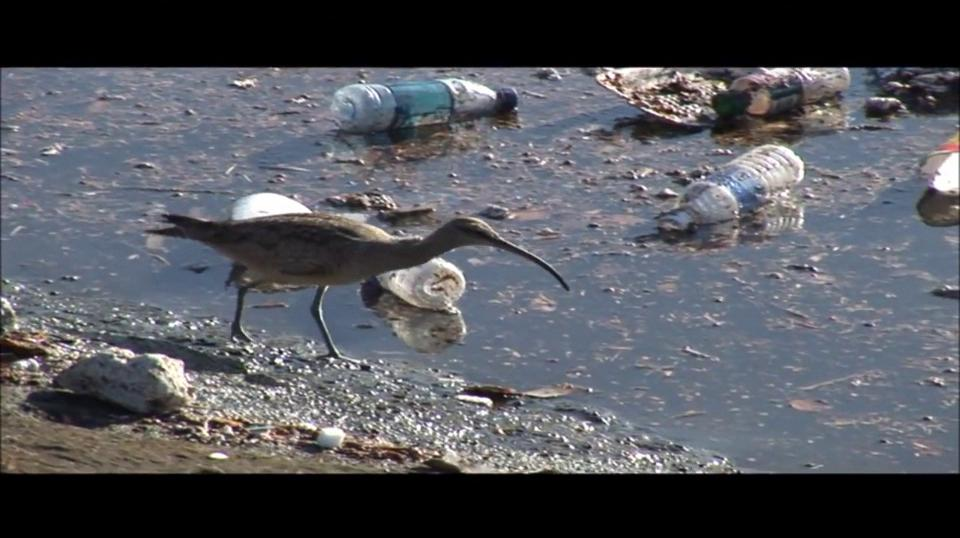
\includegraphics[keepaspectratio=true,width=.5\textwidth]{images/9077_11.jpg}
\caption{Images from the data set. Width plastic (top), width marine life (middle) and width both (bottom)}
\label{fig:plastic-data}
\end{figure}


The collected and annotated dataset is small, compared to datasets used in the training of CNNs. Therefore, as stated in the problem definition, a pre-trained network will be used. The last layer of this pre-trained network will be replaced with a layer trained on the dataset of this project.

The dataset is pseudo-randomly divided in a train(70\%), validate(10\%) and test(20\%) set. The images will be classified with the pre-trained CNN, after which the output of the second to last layer will serve as input for the small network that will be trained in this project.

The framework that will be used in this project is caffe \citet{jia2014caffe}. This framework makes it possible to test and train CNNs as well as use pre-trained networks. The interface with \texttt{Python} programming language makes it possible to combine the processing of the data with the CNN.

The accuracy of the network can be measured from the data annotations. When the network with the layer trained on the domain-specific data performs satisfactory as assumed, the detection on sub-image level will start. To classify on sub-image level more annotation will be needed to evaluate the results. However, due to the limited time this project has, the sub-image labelled data will not be made from the full dataset.

If the baseline of the CNN is not satisfactory as assumed, other imagery techniques will be used like SIFT \citet{ai2010color}, fisher vectors \citet{sanchez2013image} and local binary descriptors \citet{zhang2010local}.


\section{Plan}
Table \ref{tab:plan} and figure \ref{fig:plan} show the current planning of the remaining project.

\begin{table}[h!tb]
\centering
\caption{The plan for the remaining weeks}
\label{tab:plan}
\begin{tabular}{|p{.1\textwidth}|p{.8\textwidth}|} \hline
week & work to be done \\ \hline \hline
17 & make project plan, test first classification with caffe, get output of second-to-last layer and save for further use\\ \hline
18 & make a network to train a last layer with as input the saved data from the previous week \\ \hline
19 & train and test the made layer, use the validation set to fine-tune the network \\ \hline
20 & study trip to Edinburgh, read papers for deeper understanding of CNNs \\ \hline
21 & process the images to train on sub-image level, annotate several of the sub-images for training and testing\\ \hline
22 & test the sub-images, prepare for the half-time presentation\\ \hline
23 & refine the network for sub-images\\ \hline
24 & classify the sub-images\\ \hline
25 & test final conclusions\\ \hline
26 & writing it all down in a thesis\\ \hline
27 & finishing up \\ \hline
\end{tabular}
\end{table}

\begin{figure}[h!tb]
\centering
\xymatrix{
        {\begin{array}{l}
            \text{Collect and annotate data} \\
            \text{Install CNN framework}
        \end{array}} \ar[d] & \\
        {\begin{array}{c}
            \text{Classify last layer of CNN}\\
            \text{(2 weeks)}
        \end{array}} 
        \ar[d]_{baseline}^{satisfactory} \ar[dr]^{baseline}_{not\;satisfactory}
        & \\
        {\begin{array}{c}
            \text{Classify on subimage} \\
            \text{(4 weeks)}
        \end{array}}
        \ar[dr] & 
        {\begin{array}{c}
            \text{Use other texture-based techniques} \\
            \text{(4 weeks)}
        \end{array}}\ar[d] \\
        & 
        {\begin{array}{c}
            \text{Write report} \\
            \text{(2 weeks)}
        \end{array}}
        }
\caption{A graphical representation of the planning of the project}
\label{fig:plan}
\end{figure}

\vfill
\bibliographystyle{abbrvnat}
\bibliography{Tex_sources/bib}
\end{document}